\documentclass[runningheads,a4paper]{llncs}

\usepackage{amssymb}
\usepackage{titlesec}
\setcounter{tocdepth}{3}
\setcounter{secnumdepth}{3}
\usepackage{graphicx}
\usepackage{hyperref}

\hypersetup{
    colorlinks=true,
    linkcolor=blue,
    filecolor=magenta,      
    urlcolor=blue,
}

\begin{document}

\mainmatter  % start of an individual contribution

% first the title is needed
\title{Why OpenStreetMap and Open Government Data integration is unfeasible?}

% the name(s) of the author(s) follow(s) next

\author{Gabriele Orazi\\
Mat. 205091
\mailsa\\gabriele.orazi@studenti.unitn.it\\}
\authorrunning{Why OpenStreetMap and Open Government Data integration is unfeasible?}
% (feature abused for this document to repeat the title also on left hand pages)

% the affiliations are given next; don't give your e-mail address
% unless you accept that it will be published
\institute{
University of Trento\\
Department of Information Engineering \& Computer Science\\
Privacy \& Intellectual Property Rights course, final paper
}

\maketitle

\begin{abstract}
OpenStreetMap is a growing reality which represents the strength of crowdsourcing of geodata. The conjunction of that platform with the Open Government Data movement, which is growing too in the last decade, could generate an impressive public database that can be used by third parties to improve the lives of citizens all around the world.
Nevertheless, this result still seems to be just a daydream. Are licensing conflicts the real main reason for the problem?
%The abstract should summarize the contents of the paper and should
%contain at least 70 and at most 150 words. It should be written using the
%\emph{abstract} environment.
\keywords{OpenStreetMap, licensing conflicts, CC BY, ODbL, Open Government Data, Open Data, Bologna}
\end{abstract}

\section*{Introduction}
Since the dawn of mankind, humans have felt the need to put on paper, as faithfully as possible, the distinctive features of every corner of the globe. That role was always assigned to men of culture, figures with a huge background who have spent a large amount of their life tracking edges of fields and traveling all around the world.
Analyzing the mapping process under a philosophical perspective, experts sometimes courageously claims that mapping is more interesting than the territory itself\cite{caquard2013cartographyI}.
More complex systems have been developed during the ages, always reserving a certain fascination for the most passionate to this practice.

Nowadays, the methods have been completely overturned. Thanks to technology, anyone can contribute to the enrichment of maps, integrating as much information as possible. This is the case of OpenStreetMap, a project that aims to collect and make available as much detailed and relevant information about places, roads, monuments and buildings.
But the potential does not stop at the simple mapping: the information collected can give rise to thousands of possible uses.
Since also small contributes need to be considered as relevant information, the concept of \textit{license} need to be taken into account.
In this paper, adopted licenses will be the main subject, as necessary as, often, problematic concerning the openness linked to the open data trend. This topic has been widely discussed as a tool to create value, but in real-life, a long way need to be covered to reach the maximum potential.

In the first chapter, OpenStreetMap ecosystem will be evaluated, focusing the attention on the process used to acquire data from the community. In the second section, licenses used by OSM in the past and today will be reviewed. Lastly, in the final chapter, an attempt of analysis has been produced in order to understand why and how licenses can still be the objective of discussion for what concern the integration of Open Government Data, by administrations, and OSM database, to create a centralized source of public and free geospatial database.

\section{OpenStreetMap}
As mentioned in the introduction, one of the main actors discussed in this paper is \textit{OpenStreetMap} (\textit{OSM})\cite{haklay2008openstreetmap}, a powerful platform in continuous evolution that relies on a strong and passionate community, which is the one of the best worldwide representation of a crowdsourced project\cite{chilton2009crowdsourcing}.
OSM is an open-source project, started in 2004, with the aim of collect and freely provide geospatial data to anyone.

\subsection{Parties inside the organization}
The \textit{foundation} (OSMF) that stands beside the project is an international non-profit that wants to follow the developments of the project, encouraging the growth and distribution without controlling or managing OSM. It's important to emphasize that the community is the heart of the project, leading the entire development process.

\textit{Volunteers} are organized in development groups, even if the components decided to participate for such different goals: for someone can be an hobby, for others it's just a matter of enriching a particular area that they evaluate as relevant, but there's space also for who thinks that OSM could be crucial in case of geological crisis such as earthquakes and tsunamis.

\textit{Groups} are used to organize the so-called ``\textit{mapping parties}'', in which volunteers meet each other with the aim of mapping all together a specific uncovered area. These events are also the springboard to attract new volunteers who espouse the cause and, for sure, instruct them on how the OSM's process works.

It's impressive to see how the effort behind the project is spread between such different realities: as well explained in \cite{haklay2008openstreetmap}, the OSM community is composed by passionate individuals but they're supported by different organizations such as states and even different private companies.

\subsection{Growth and diffusion}
Nowadays OSM is one of the reference points for geospatial services, along with Google Maps, Bing Maps and MapBox. Although the project was launched in the first lustrum of 2000, it experienced strong growth in the first half of 2012.
In fact, us reported by BBC\footnote{Google Maps to charge for usage, \href{https://www.bbc.com/news/business-15523050}{BBC}, 31 October 2011.}, Google announced in October 2011 the intent to introduce a fee for services that rely on Google Maps API, starting from April 2012. Going deeper into the details, the fee is only charged for services that make intensive use of the API, recording more than 25,000 map hits per day. Together with the announce, Google reported that, according to their projections, only 0,35\% of users would have been involved in the tariff change. Google has reserved the right to publish the real impact of their policy, leaving to this percentage irrelevant importance from a statistical point of view, but rather just using it for the marketing side.
What is important after the actuation of this policy is the effects that have been generated for the competitors: OSM gained the most, thanks to his accuracy and, most important, his concept of open-source data.
The growth can be supported by the graph in figure \ref{fig:osm_users}\footnote{OpenStreetMap Wiki, \href{https://wiki.openstreetmap.org/wiki/Stats}{Stats section}.}, in which is easy to notice how many users started to join the community, establishing a positive trend that still today seems to be constantly growing.
It's interesting to notice how companies that push on open source philosophy, as well as others that do not, decided to migrate to OSM.
Wikipedia was one of the first organizations that jumped in\footnote{Wikipedia updates mobile apps, drops Google Maps for OpenStreetMap, \href{https://www.theverge.com/2012/4/7/2931320/wikipedia-updates-mobile-apps-drops-google-maps-for-openstreetmap}{TheVerge}, 7 April 2012.}: for obvious reasons, the two sides find many points of contact, where surely emerges the concept of community on which the two services are based.

Even private companies decided to trust the open-source movement, adopting OSM after years of Google Maps usage: this is the case of Foresquare and StreetEasy\footnote{After price hike, Foursquare and StreetEasy switch from Google to OpenStreetMaps, \href{https://venturebeat.com/2012/03/01/google-maps-api-price-foursquare-streeteasy-openstreetmaps/}{VentureBeat}, 1 March 2012.}, which decided to migrate in favor of the open service, with a higher level of customization and design flexibility.

Today OpenStreetMap is used by many huge companies such as Facebook, Amazon, Apple, Microsoft, Pinterest, Snapchat and Uber as well as so many different governments, universities (Cambridge is just one instance) and news and media agencies\footnote{OpenStreetMap Wiki, \href{https://welcome.openstreetmap.org/about-osm-community/consumers/}{Who uses OpenStreetMap?}}.

\begin{figure}
    \centering
    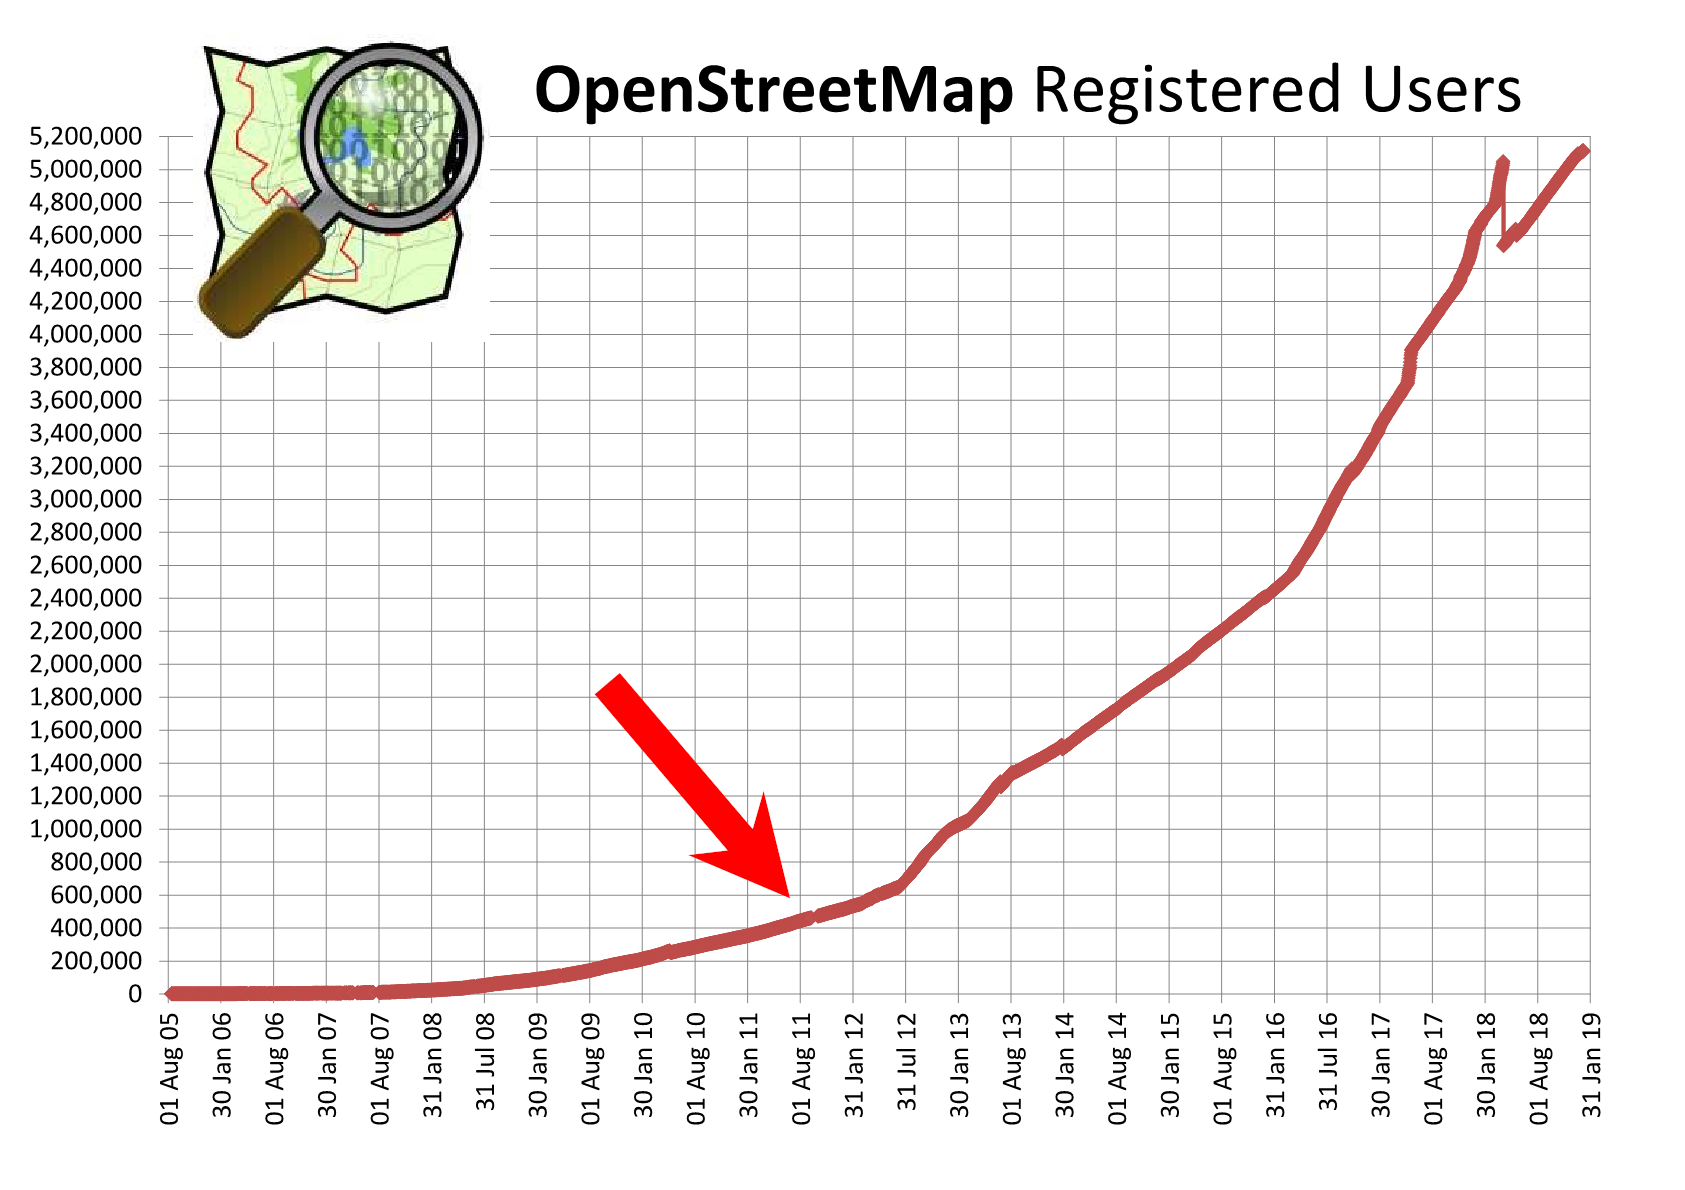
\includegraphics[width=0.9\linewidth]{images/osm_registered_users.png}
    \caption{OSM Accumulated registered users}
    \label{fig:osm_users}
\end{figure}

Another relevant point of discussion is the accuracy and coverage of the mapping data across different services, all with the same purpose. Different approaches has been studied to understand points of divergence and causes that stand behind those. 5 different cities in Ireland have been taken into account in a study\cite{ciepluch2010comparison}. The paper outcome is noteworthy: in comparison, Google Maps and OSM accuracy seems to be equal, underlining how far a community-based project can go. The sticking point of the comparison is the coverage: important areas are well-mapped, but, differently
from Google Maps, OSM lack in peripheral coverage.
The author of the study used to describe the phenomenon as ``\textit{areas where nobody wants to map}". In fact, this description traces perfectly where the point of the discussion is: Google has a relevant advantage with respect to OSM because is a private organization that doesn't rely on the community's needs.
This problem has been noticed also by Caquard S.\cite{caquard2014cartographyII}, which states that, despite the significant improvement that mapping communities have made over the years, inequalities persist in terms of geospatial contribution.
This is still representing the major obstacle for OSM development in the long run.

\subsection{Imports}
Before digging into adopted licenses and related issues, is worthy to analyze how new data is processed in order to be inserted into the database, and consequently, be available for the final user.

\subsubsection{Control entities: DWG \& LWG}~\\ \newline
In the \textit{import} process, two entities, both authorized by the OSMF, play crucial roles:
\begin{itemize}
    \item The \textbf{Data Working Group}\footnote{\href{https://wiki.osmfoundation.org/wiki/Data_Working_Group}{DWG official wiki}.} (DWG) is the authority that provides integrity on stored data. It handles user's complaints and regulates discussions and disputes that can come up in decisions taken by the community. It also has decision-making power in case of vandalism detection, asking to the \textit{Operations Working Group} (OWG) to ban or limit the usage of APIs for a certain IP address and even deleting all diary entities.
    \item The \textbf{Licensing Working Group}\footnote{\href{https://wiki.osmfoundation.org/wiki/Licensing_Working_Group}{LWG official wiki}.} (LWG) is responsible for all licensing issues related to geodata: creation of new contents, following the \textit{import} process, need to be regulated and pass through licensing controls, as well as correct usages of provided information (end-user license).
    The team is also in charge of handling possible copyright infringement raised by intellectual property owners, as well as all other possible disputes such as child protection, privacy, trademarks and so on.
\end{itemize}
OSM is composed by some other working groups that are missing here, but since these two are the most important ones for this work, it's been decided to overcome the description of each group that composes the organization.
By the way, it's important to notice that all the different groups are always composed by a restricted number of community members that for a long time have contributed to the development of the project.

\subsubsection{Import processing}~\\ \newline
The \textit{Import} is the procedure to follow by which community can add their contributes in the database.
At first, it's hardly recommended to discuss with the community before start working on the data collection: a certain kind of information could be useful in a specific area, rather than in another city in which is not relevant at all. It's important to notice that the community (distributed inside a hierarchical organization, starting from countries till local groups) should approve your plan and can simply deny accepting the submitted work at this very first stage.
Depending on the complexity and scale of the import, the DWG can ask for technical assistance of some experienced OSM volunteers.
After passing this early stage, license approval needs to be taken into account. Permissions and licenses need to be obtained from the data owner. Most important, all licenses need to be complied with \textit{Open Database License} (ODbL) in order to be uploaded and used in OSM platform (more on ODbL in section \ref{sec:licensechange}).  
This is a crucial point of interest for this study: obtain licenses, in most of the cases, appears to be the hardest task to be accomplished because of policies that may be in use depending on localities and organizations. Still, this one of the main reason why the majority of license conflicts came out. Policies can be almost open but still having conflicts or, for instance, could have restrictions for commercial use or attribution requirements.
The LWG, as the guarantor of this delicate phase, provides volunteers with templates to expressly request to data owners if they are willing to comply with the OSM ODbL terms.
After accomplishing this awkward phase, the volunteer must document how he is planning to complete the import. Raw data need to be converted into OSM XML format and be handled in such a way that permit to simplify and, at the same time, be more informative as possible. The user is not alone and should mention in the documentation other volunteers to split the work.
Before start the provided plan, the documentation needs to be submitted for the final review, made by different delegations of the foundation (of course DWG and LWG take part in the review). Only when a confirmation will be sent back, the import can be finalized realizing the plan, tracking progresses to the community till the end of all the procedures.

\section{OSM and licenses}
In an open-source project such as OSM, licensing is one of the most important aspects to take in consideration.
Even if the philosophy behind the open-source concept could appear trivial, the reality is slightly different: plenty of licenses has been released to shape in the best way as possible different needs and to satisfy every creator that decided to share something.
More than for single creators, companies and organizations find difficult to share information in public because of different motivations that can differ a lot concerning the environment that surrounds the company itself.
A framework has been traced to analyze and understand why and what sustains the need of so many different policies: in the proposed paper\cite{zuiderwijk2014open}, the Dutch governmental organization has been chosen as a case study.
The outcome underlines that, even if a lot of organizations would like to be more open, clearly seen the real potential, there's another huge slice of institutions that see open data as a threat in terms of legal liability, data misinterpretation and also reputation damage.
With this assumption, it's easy to understand how the process that needs to be taken is long and divided into so many different steps that go hand-by-hand with how and how much data an organization is willing to share.
This, for sure, is the main reason that fires the proliferation of so many licenses variance: in most of the cases, such the one taken into account in the following chapters of this paper, the result is \textit{license conflicts}. When a similar situation occurs, suddenly all the spent effort and the strength of open data lose his power.

OSM, one of the biggest open database, has and had to deal with licenses and related \textit{intellectual property} behind managed information. In April 2010, the organization has made a big step, changing retrospectively the used license and implementing what was published a few months earlier in the new license proposal\cite{amos2009new}. The way how this change has been managed is interesting because required to collaborators to accept new terms imposed by the entry license. In next sections an extensive analysis.

\subsection{Change of license: from CC\_BY-SA to ODbL}\label{sec:licensechange}
Despite the decision of switching license, OSM didn't change at all for the final user. All the changes have been transparent from the outside, but actually, the change has been receipted by contributors, especially the old ones.
The new and the old licenses (ODbL and CC\_BY-SA respectively) enable a similar usage of OSM data but despite the old license,
ODbL best suits the needs of the open data collected in the open database.

\subsubsection{Why OSM changed license}~\\
The last used version of CC\_BY-SA was 2.0. The biggest issue is that the license, as well as all the other versions, is not designed to suit the needs of data collected into a database. Even the Creative Commons (the authority that stands behind CC\_BY), before publishing the version 4.0, reported the incompatibility\footnote{Quote cited in OSM wiki, no more available because of version 4.0 of CC\_BY-SA.}:
\begin{quote}
    \textit{Creative Commons does not recommend using Creative Commons licenses for informational databases, such as educational or scientific databases.}
\end{quote}
Analyzing the weaknesses of CC\_BY-SA listed in \cite{OSM2010why}, it is reasonable to justify the change:
\begin{itemize}
    \item The concept behind \textit{copyright} is perceived completely different depending on jurisdictions: for instance, US considers \textit{information} not copyrightable because of the willing to encourage progress on science and art. The creative expression is the key that distinguishes the intellectual property from simple information. Totally different vision is adopted in the UK, in which copyright is possible simply demonstrating the effort of persons collecting information.
    Remembering that CC\_BY-SA completely relies on copyright concept and combining what just explained regarding different perspectives of jurisdictions, it's possible to claim that OSM data cannot be protected by CC\_BY-SA.
    \item Producing a new item, combining a CC\_BY-SA licensed data (for example an OSM map) with another piece of data with no specific license will require to obtain CC\_BY-SA compatibility for the additional data. This makes too difficult (or impossible) to use certain data sources in OSM rendered maps.
    \item The \textit{Share Alike} concept, introduced with GPL\footnote{GNU General Public License.} by Richard M. Stallman in the open-source and free software context\cite{carver2005share}, impose to who is using OSM data producing something, to share it with CC\_BY-SA license. That will allow, hypothetically, Google to integrate OSM data in their systems, to create and release a painting but, at the same time, to keep hidden the improved data used to create the painting, avoiding to share it.
    \item CC\_BY-SA comes with an \textit{attribution} obligation, which means that any usage of data should mention all contributor names that stand behind. This has been ignored for ages in OSM because of the practical impossibility of fulfillment, but, actually, it can retain publishers from outside the community to avoid the usage of such data because of they may be blamed of copyright infringement.
\end{itemize}
The conjunction of all those issues pushes the community to jump in ODbL, which required much effort but which, in one shot, solved many points that otherwise would have been difficult to solve individually.

\subsubsection{How OSM changed license}~\\
The transaction between one license to the other may be perceived as a simple step to been accomplish, but actually, for OSM it's been more arduous than what expected.
The process took more than two years and required to interact with all the contributors (active or not) to ask them permission over data that they have collected before.
Each community component was asked to accept the new terms. This decision confronted the subject with different choices: \textit{accept} new license terms, which means re-license the past contributions under ODbL license, or \textit{decline} the proposal, denying to OSM to use the contributions and, consequently, to the entire OSM user population.
If the person had decided to accept the terms, another decision would have had to be taken. The user could both decide to \textit{maintain} the CC\_BY-SA license, continuing to be personally attributed to the work carried out or to consider all contribute \textit{Public Domain}. Legally, the decision had the same value but, ideally, this would have been an important thought towards the open philosophy that distinguishes OSM. Luckily, the community has shown that it is in line with the new policies: in fact, as reported by the OSM itself\footnote{Information taken directly from the \href{https://wiki.openstreetmap.org/wiki/Open_Database_License}{OSM Wiki}.}, only 1\% of the geodata were lost during the transition.

The license change represents the transition from a \textit{federal copyright system}, in which thousands of contributors need to be asked for each license issue, to a \textit{centralized} one, where instead OSM has the power to be considered as a single licensor. Thanks to this, OSM can control and handle all contents properly and easily for future developments, legally and technologically speaking. 
This is not the only point of strength: ODbL can cover the biggest CC\_BY-SA issue, represented by the concept of copyright, which has been replaced by the \textit{Sui Generis database right}\cite{ginsburg1997copyright}. Insecurity generated by a different interpretation of copyright made by jurisdictions can be avoided and solved thanks to the possibility to recognize the investment that has been made in compiling a database, even if no creativity process has been involved.
Lastly, even the \textit{Share Alike} issue has been solved. Indeed, ODbL permits to create new contents even when licenses incompatibilities in data sources are present and, most important, impose to share any enhancement that has been performed in the creation of the new content.



\section{License conflicts: breaking OSM potential}
Despite a large amount of data in which OSM can count on thanks to the active community, the strength of the project can be maximised only when data is integrated by third-party data sources. Indeed, different sources have been used by the organization in order to double-check, enrich and improve already collected data.
OGD movement can represent a perfect subject to integrate inside OSM project, which can hypothetically lead to think to a single, open and public integrated platform at the service of all world-wide citizens.
Thus, try to integrate and different licenses applied on different sources is still a challenge for the LWG and the community itself, representing again the biggest boundary to overcome.

\subsection{Open Government Data}\label{previous}
In the last decade, the concept of \textit{Open Government Data} (OGD) is taking place in different countries. As explained and analyzed in \cite{ubaldi2013open}, OGD is a sort of movement with the aim of convincing different administrations (from the local one since an entire country) to develop and provide web portals and APIs for the benefit of all, to improve and create new services that can generate value for the citizen.

In \cite{jetzek2013generating}, 61 countries have been taken into account with the goal of finding a correlation between the welfare of a certain population and the ``openness" of the respective administration: the outcome underlines how OGD can effectively create value, from the health and wellbeing to the environmental, passing through education and even GDP monetary value.
Four major factors have been evaluated as the fundamental concepts that automatically feed the entire process of OGD, increasing more and more the created value:
\begin{itemize}
    \item \textit{Efficiency}, improving resource allocation which can be practically translated into improving administrative bureaucracy, cutting processing costs, sign agreements with other countries and so on;
    \item \textit{Innovation}, generated by the proliferation of new services on top of the shared data;
    \item \textit{Transparency}, cutting corruption and unfair competition between different parties;
    \item \textit{Participation}, creating a prolific field where to add experience and ideas to solve difficult social problems.
\end{itemize}

\subsection{Barriers of the integration}
Unfortunately, on top of all those good intentions, not all countries are yet able to grasp the potential.
Despite the multitude of references that praise the OGD movement, in \cite{janssen2012benefits} the fairy tale has been criticized, analyzing the scenario under a practical and disillusioned point of view. In the paper, authors underline how governments are still afraid of the new trend and even if some steps have been done, this is not enough to honor promises explained in \ref{previous}. Governments should just accept to lose some degrees of control over their data, otherwise what released is no more than mere and useless advertisement to sponsor how transparent and open an administration is. Open data need to be taken into account discussing the entire infrastructure, improving quality of datasets which, in most of the cases, are poor and pretty unusable, and developing into users and citizens a "sense of data", ensuring public engagement.

Moreover, also in this scene, licenses could represent a big barrier that can further drain the usability of shared data.
Indipendently from the kind of shared data, each administration decides also which license to apply on top of released information.
Most used license is, again, Creative Commons. Even \textit{European Data Portal}, the platform developed by the European Union with the aim of collecting all open data provided by the 28 European Member States and four EFTA countries\footnote{The European Free Trade Association (EFTA) is a regional trade organization and free commerce area composed by four European states: Iceland, Liechtenstein, Norway, and Switzerland.}, strongly suggest to provide public sector information under CC\_BY licenses\footnote{\href{https://www.europeandataportal.eu/elearning/en/module4/#/id/co-01}{European Data Portal} page related to licensing.}.

Beyond the described issues and criticisms over OGD movement, the idea of integrating such open datasets let imagine OSM as a great opportunity to maximize the potential of both involved parties.
On one hand, OSM would see an exponential increase in the amount of available data, potentially becoming the largest open database that goes so far beyond the simple geospatial service. On the other hand, the OGD movement would become extremely valuable in a context where developers (not only private individuals but also large corporations) could benefit more and more.
So, why was this integration never even considered? For sure, legal issues linked to licenses represents again one of the biggest obstacles to overcome.

LWG, together with CC\_BY, spent a lot of effort to try to find a way to handle licenses without explicitly ask for new permissions to different contributors to the involved data sources. Unfortunately, they fail to solve the problem, leaving the mandatory obligation to let the contributor waive over attribution and unrestricted distribution of data.
OSM Wiki provides an exhaustive table\footnote{OpenStreetMap Wiki, \href{https://wiki.openstreetmap.org/wiki/Import/ODbL_Compatibility}{ODbL compatibility table}.} in which all licenses are listed together with compatibility and, in case of collision, required waivers to been obtained. Confirming that table, in \cite{khayyat2015open} a similar study of incompatibility between ODbL and CC\_BY licenses has been confirmed in between a more extensive analysis, proposing CC0 as a good alternative for ODbL.
CC0 is fully compatible with OSM because of the complete rights waive in favor of the public domain. So actually, this license can potentially solve all license inconsistencies but is not used at all by governments. Furthermore, it's trivial to understand that administrations are not so keen to adopt a kind of license that grants a copyright waiver for all their data.

This \textit{deadlock state} blocks every possible efficient and profitable development. CC0 is the practical solution to feed both OSM and public added value growth, but governments are still reluctant to make the required divestiture.  

\subsection{Wrong approaches: Bologna's case of study}
Trying to analyze the types of licenses used by different cities that have decided to share datasets, Bologna can certainly be represented as an excellent case study.
The municipality decided to apply a CC\_BY 4.0 license over a multitude of datasets, including libraries, schools, cycle paths and so on. There are also a lot of 3d-models of the most famous and historical buildings and monuments of the city.

Unfortunately, as already explained, the used license is the reason why, looking for Bologna from OSM website, the city seems to be comparable to any other place that is not active at all for what concern open data. Since is a big and important city, point of interest are well indexed but is clearly noticeable that municipality open datasets are not involved in OSM.
But the most important and relevant point is the strange behavior that Bologna's administration decided to adopt: from the Bologna's Open Data portal there is a webpage dedicated to adopted licenses\footnote{Bologna's Open Data website, \href{http://dati.comune.bologna.it/node/3449}{CC BY 4.0 ODbl compliant}.}, in which is possible to find an addendum.
The clause is a waive in favor of OSM for what concern the ``\textit{Ortofoto Bologna}" dataset, in line with permissions that OSM ask for in its cover letter\footnote{\href{https://wiki.openstreetmap.org/wiki/CM/en/001_-_Cover_letter_and_waiver_template_for_CC_BY_v4}{OSM Cover email} to ask for necessary waives in case of CC\_BY 4.0 license.}.
Such an email template is provided to community's components to ask third party data owners to allow the incorporation of CC\_BY 4.0 data into OSM.

This is a clear bad example of ad hoc license, creating an impartial situation in which is difficult to find out a clear understanding of the meaning that stands behind that decision.
The impression gained during the study of these dynamics leads to think of a behavior reluctant to assume responsibility, derived from the uncertainty over multiple usages that the public domain can create with respect to released data.
Governments and administrations reserve the right, in so doing, to be blamed for hypothetical bad habits, avoiding also any mended interventions required to fix the scenario, overcoming the fact that this approach is a serious blow to the transparency and intrinsic ethics of open data.   

\section{Conclusions}
In this paper, a complete analysis has been carried out regarding the licensing system adopted by OpenStreetMap, the guidelines adopted by the various public administrations that adhere to the Open Government Data movement, as well as the possible barriers (voluntarily erected or not) that legal concessions can create.
Despite the growing enthusiasm of recent years, which has come to create compared to the much-vaunted concept of OpenData, projects like OSM still struggle to leave the nest because of scary jurisdictions, which are claiming to be part of the OGD movement, but still struggle to fully embrace open politics in the reality.
Finally, a representative example has been taken into consideration: the municipality of Bologna, with its Open Data portal, represents the timid attempt to grant, with a clause on the current license incompatible with OSM, only a small dataset to the public domain compared to the multitude of data that could be lifeblood for the proliferation of new services and improvement of existing ones.   

\newpage
% bibliography in bibtex format
% adding chapter to index
\addcontentsline{toc}{chapter}{Bibliography}

% style with alphabetical order wrt authors
\bibliography{biblio}
\bibliographystyle{unsrt}

\end{document}
